\section{Question 1}

\begin{question}
     Learn a Decision Tree from the whole dataset by setting the minimum gain threshold to 0.01, while
keeping the default configuration for all the other parameters.

     \\
     a: Which attribute is deemed to be the most discriminative one for class prediction?
     \\
     b: What is the height of the Decision Tree generated?
     \\
     c: Find a pure partition in the Decision Tree and report a screenshot that shows the
    example identified.
\end{question}
\begin{anwer}
     a: The most discriminative attribute is \textbf{node-caps} which is found at the root of the
     decision tree. If the classifier just take into account \textbf{node-caps}, it clasifies as the bottom image shows.

     \begin{center}
          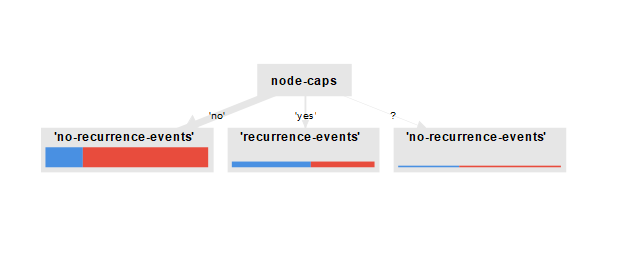
\includegraphics[width=0.8\textwidth]{Screenshot_1.png}
        \captionof{figure}{Decision Tree with just node-caps as input.}
    \end{center}
     \\
     With an accuracy of \textbf{0.72}, and for:
     \\
     \textbf{non-recurrence-events} a recall of \textbf{0.87} and precision of \textbf{0.76}
     \\
     \textbf{recurrence-event} a recall of \textbf{0.36} and precision of \textbf{0.55}.
     \\
     \linebreak
     b: The max height of the decision tree generated is: \textbf{5} and the min height is: \textbf{2}.
     \\
     \linebreak
     c: At the bottom, an image of a pure partition can be found. It follows the path:
     \\
     node-caps(yes) -> deg-mailig(3) -> breast(right) -> irradiat(yes) for a no-recurrence-events class.
     \\
     The particular in this path is that the other
     paths shown for recurrence-events are also almost pure.
     \\
     \begin{center}
          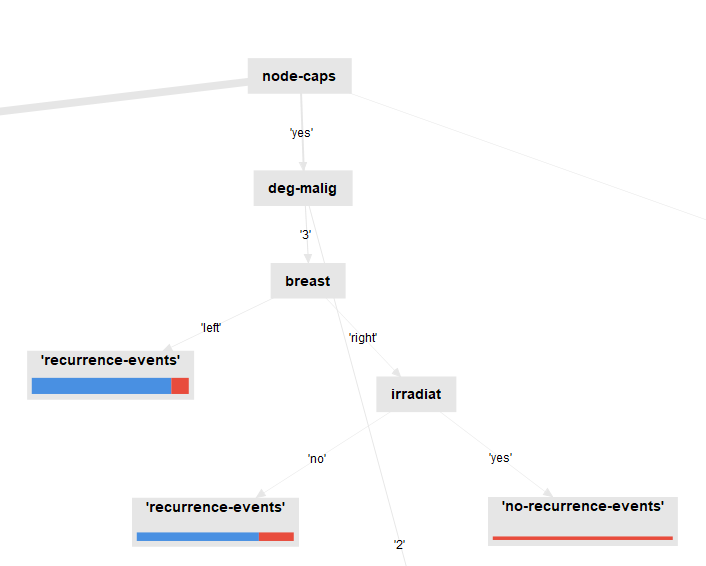
\includegraphics[width=0.8\textwidth]{Screenshot_2.png}
          \captionof{figure}{Pure partition from Decision Tree model.}
     \end{center}
\end{anwer}
\pagebreak